% Standalone Beamer lecture. Compile twice with pdflatex.
% Source sequence: Notesweek4.pdf (pp. 1-10), Notesweek5.pdf (pp. 1-6), Notesweek6.pdf (pp. 1-13).
\documentclass[aspectratio=169,11pt]{beamer}
\usepackage[T1]{fontenc}
\usepackage{lmodern,amsmath,amssymb,bm,booktabs,tikz,pgfplots,listings}
\usetikzlibrary{arrows.meta,positioning}
\pgfplotsset{compat=1.18}
\definecolor{ink}{HTML}{173754}
\definecolor{sea}{HTML}{007478}
\definecolor{warm}{HTML}{AA4C2A}
\setbeamercolor{normal text}{fg=ink,bg=white}
\setbeamercolor{structure}{fg=sea}
\setbeamercolor{frametitle}{fg=ink}
\setbeamercolor{alerted text}{fg=warm}
\setbeamerfont{frametitle}{series=\bfseries}
\setbeamerfont{title}{size=\LARGE,series=\bfseries}
\setbeamercolor{title}{fg=ink}
\setbeamertemplate{navigation symbols}{}
\setbeamertemplate{itemize items}[circle]
\setbeamertemplate{footline}{\hspace{6mm}\raisebox{2mm}{\scriptsize\color{sea}\insertsectionhead}\hfill
\raisebox{2mm}{\scriptsize\color{ink}\insertframenumber/\inserttotalframenumber}\hspace{6mm}}
\setbeamersize{text margin left=7mm,text margin right=7mm}
\setlength{\parskip}{0.37em}
\newcommand{\R}{\mathbb R}
\newcommand{\vct}[1]{\bm{#1}}
\newcommand{\norm}[1]{\lVert #1\rVert}
\newcommand{\diag}{\operatorname{diag}}
\newcommand{\src}[1]{\par\smallskip{\scriptsize\color{gray}#1\par}}
\newcommand{\four}[1]{\src{Week 4 handwritten notes, #1.}}
\newcommand{\five}[1]{\src{Week 5 handwritten notes, #1.}}
\newcommand{\take}[1]{\par\smallskip{\color{sea}\bfseries #1}\par}
\lstset{language=Python,basicstyle=\ttfamily\small,keywordstyle=\color{ink}\bfseries,
commentstyle=\color{sea},stringstyle=\color{warm},showstringspaces=false,
columns=fullflexible,keepspaces=true}
\tikzset{state/.style={draw=ink,minimum width=1.1cm,minimum height=0.64cm},
edge/.style={-{Latex[length=2mm]},thick,ink}}
\title{Convolutional and recurrent neural networks}
\subtitle{Spatial filters, dynamical systems and backpropagation through time}
\author{Morten Hjorth-Jensen}
\institute{University of Oslo \quad FYS5429/9429}
\date{Weeks 4--6}
\begin{document}
\section{Week 5: recurrent dynamics}
\begin{frame}{Velocity supplies the missing state}
Two oscillators pass through the same position $q$ at the same time, one moving
left and the other right. Their next positions differ even if the applied force
is identical. Position alone is an incomplete description.
\[
m\ddot q+\gamma\dot q+kq=F(t),\qquad v=\dot q.
\]
With initial conditions $(q_0,v_0)$ the two first-order equations are
\[
\dot q=v,\qquad \dot v=\frac{F(t)-\gamma v-kq}{m}.
\]
Here $m$ is the mass, $\gamma$ the damping coefficient and $k$ the spring
constant. Setting $m=k=1$ gives the normalized equation of the notes.
\five{p.\ 2}
\end{frame}
\begin{frame}{Euler's method is a recurrence}
Let $t_n=t_0+n\Delta t$ and $F_n=F(t_n)$. Forward Euler evaluates \emph{both}
right-hand sides at $t_n$:
\[
q_{n+1}=q_n+\Delta t\,v_n,\qquad
v_{n+1}=v_n+\frac{\Delta t}{m}(F_n-\gamma v_n-kq_n).
\]
The velocity update can also be read as a cell that receives $F_n,q_n$ and
carries $v_n$ from the previous step:
\[
v_{n+1}=
\underbrace{(1-\gamma\Delta t/m)}_{\text{recurrent weight}}v_n+
\underbrace{(\Delta t/m)}_{\text{force weight}}F_n-
\underbrace{(k\Delta t/m)}_{\text{position coefficient}}q_n .
\]
To run the oscillator autonomously, propagate $q_n$ as well as $v_n$.
\five{pp.\ 3--4}
\end{frame}
\begin{frame}{The state-space update}
With $s_n=(q_n,v_n)^\top$, the same Euler step is
\[
s_{n+1}=As_n+BF_n,\qquad
A=\begin{pmatrix}1&\Delta t\\-k\Delta t/m&1-\gamma\Delta t/m\end{pmatrix},
\quad B=\begin{pmatrix}0\\ \Delta t/m\end{pmatrix}.
\]
After two steps,
\[
s_2=A(As_0+BF_0)+BF_1=A^2s_0+ABF_0+BF_1.
\]
Both inputs affect $s_2$, but the contribution from $F_0$ passes through an
additional application of $A$. Its influence at $s_n$ is $A^{n-1}B$.
\five{pp.\ 3--4, with the state written in matrix form}
\end{frame}
\begin{frame}{An unfolded sequence of velocity updates}
\begin{center}
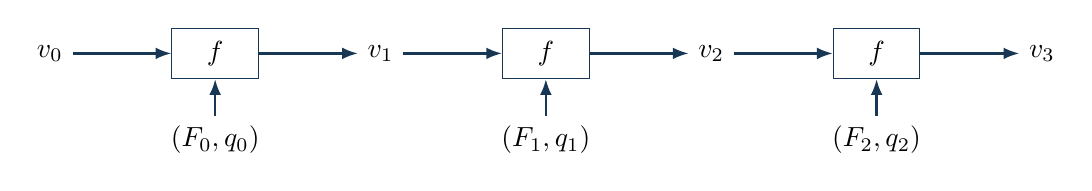
\begin{tikzpicture}[x=2.1cm,y=1cm]
\node (v0) at (0,0) {$v_0$};
\foreach \i/\j/\n in {1/0/1,3/1/2,5/2/3}{
\node[state] (f\j) at (\i,0) {$f$};
\node (x\j) at (\i,-1.1) {$(F_{\j},q_{\j})$};
\draw[edge] (x\j)--(f\j);}
\node (v1) at (2,0) {$v_1$};\node (v2) at (4,0) {$v_2$};\node (v3) at (6,0) {$v_3$};
\draw[edge] (v0)--(f0);\draw[edge] (f0)--(v1);
\draw[edge] (v1)--(f1);\draw[edge] (f1)--(v2);
\draw[edge] (v2)--(f2);\draw[edge] (f2)--(v3);
\end{tikzpicture}
\end{center}
The labels $f_0,f_1,\ldots$ in the handwritten graph mark evaluations
of the update at different steps. Here we write $f$ at every step to
emphasize that its coefficients are shared.
\par
When $q_n$ is measured, it enters as an input alongside $F_n$. When
positions are also predicted, the carried state must include $q_n$.
\five{p.\ 4}
\end{frame}
\begin{frame}{Observed velocities and a shared objective}
With measured positions and forces as inputs, let $G_\theta$ denote the full
velocity update and let $v_0$ be known:
\[
\hat v_{n+1}=G_\theta(\hat v_n,q_n,F_n),\qquad
\ell_{n+1}=\tfrac12(\hat v_{n+1}-v_{n+1}^{\rm obs})^2 .
\]
\[
\hat\theta=\arg\min_{\theta\in\R^P}\mathcal L(\theta),
\qquad \mathcal L(\theta)=\sum_{n=0}^{N-1}\ell_{n+1}(\theta).
\]
In the notes' compact drawing the loop carries the predicted velocity back
as input to the next update. In the unfolded drawing, the observed velocity
enters each loss from the other side. These are two views of one computation.
\five{pp.\ 5--6}
\end{frame}
\section{Week 6: the simple recurrent network}
\begin{frame}{The oscillator supplies a model for the hidden update}
Week 6 absorbs the mass into the coefficients. Write
$\alpha=\gamma/m$, $\beta=k/m$ and $\widetilde F_n=F_n/m$. Then
\[
v_{n+1}=v_n+\Delta t(\widetilde F_n-\alpha v_n-\beta q_n).
\]
In the velocity-fitting diagram, identify $h_{t-1}$ with $\hat v_n$ and
$x_t$ with $(q_n,\widetilde F_n)^\top$, where $t=n+1$.
The physical state update becomes a learnable rule $h_t=f_\theta(h_{t-1},x_t)$.
\par
The handwritten weights $W_{hx},W_{hh},W_{hy}$ will be denoted
$U,W,V$, respectively: input to state, state to next state, and state to readout.
The biases $b,c$ are shared across time, just like the matrices.
\src{Week 6 handwritten notes, pp.\ 2--7.}
\end{frame}
\begin{frame}{A simple recurrent neural network}
Use columns throughout. At steps $t=1,\ldots,T$:
\[
\boxed{\begin{aligned}
a_t&=Ux_t+Wh_{t-1}+b, & h_t&=\phi(a_t),\\
o_t&=Vh_t+c, & \hat y_t&=\psi(o_t).
\end{aligned}}
\]
\begin{center}\begin{tabular}{lll}\toprule
Input dimension $d$ & Hidden dimension $H$ & Output dimension $p$\\\midrule
$x_t\in\R^d$ & $a_t,h_t,b\in\R^H$ & $o_t,\hat y_t,c\in\R^p$\\
$U\in\R^{H\times d}$ & $W\in\R^{H\times H}$ & $V\in\R^{p\times H}$\\\bottomrule
\end{tabular}\end{center}
The oscillator is a linear special case with $\phi(a)=a$, $W=A$, $U=B$
and $x_t=F_{t-1}$. A nonlinear hidden state need not coincide with $(q,v)$.
\src{Week 6 handwritten notes, pp.\ 5--7, expanded in column-vector notation.}
\end{frame}
\begin{frame}{The readout gives each step a path to its loss}
\begin{center}
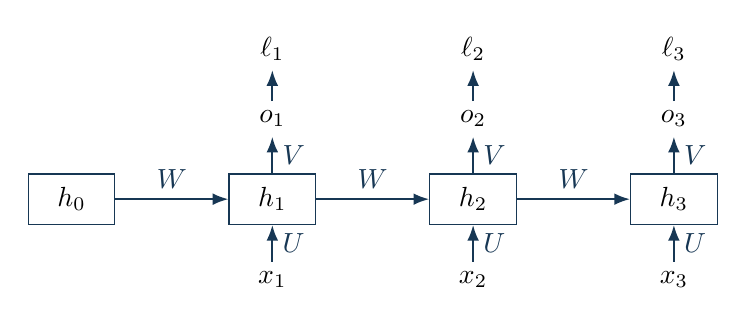
\begin{tikzpicture}[x=2.55cm,y=0.85cm]
\node[state] (h0) at (0,0) {$h_0$};
\foreach \t in {1,2,3}{
\node[state] (h\t) at (\t,0) {$h_\t$};
\node (x\t) at (\t,-1.2) {$x_\t$};
\node (o\t) at (\t,1.2) {$o_\t$};
\node (l\t) at (\t,2.25) {$\ell_\t$};
\draw[edge] (x\t)--node[right] {$U$}(h\t);
\draw[edge] (h\t)--node[right] {$V$}(o\t);
\draw[edge] (o\t)--(l\t);}
\draw[edge] (h0)--node[above] {$W$}(h1);
\draw[edge] (h1)--node[above] {$W$}(h2);
\draw[edge] (h2)--node[above] {$W$}(h3);
\end{tikzpicture}
\end{center}
Each occurrence of $U$, $W$ or $V$ represents the same parameter. The compact
cell has a recurrent loop; its unfolded computation has no directed cycle.
\src{Week 6 handwritten notes, pp.\ 4--7. Each loss also receives its observed target.}
\end{frame}
\begin{frame}{The sequence loss determines where errors enter}
Let $\ell_t=\ell(\hat y_t,y_t)$ and fix nonnegative weights $\alpha_t$:
\[
\mathcal L(\theta)=\sum_{t=1}^T\alpha_t\ell_t,\qquad
\theta=(U,W,V,b,c).
\]
\begin{center}\begin{tabular}{ll}\toprule
Per-step supervision & $\alpha_t=1$ for a sum, or $1/T$ for a mean\\
Final-time supervision & $\alpha_T=1$, all earlier $\alpha_t=0$\\
Partially labeled sequence & $\alpha_t=0$ where a target is missing\\\bottomrule
\end{tabular}\end{center}
Unless stated otherwise, $h_0$ is fixed. An unlabeled early step still influences
a later labeled step through the hidden state.
\src{Week 6 handwritten notes, pp.\ 5--7, extended to weighted and final-time losses.}
\end{frame}
\section{Week 6: backpropagation through time}
\begin{frame}{Two paths out of a hidden state}
At $h_t$ there are two departures in the unfolded graph:
\[
h_t\longrightarrow o_t\longrightarrow\ell_t,\qquad
h_t\longrightarrow h_{t+1}\longrightarrow\text{later losses}.
\]
Call the \emph{direct} derivative from the local readout $q_t$ and the
\emph{total} derivative from all reachable losses $g_t$:
\[
q_t=\nabla_{h_t}(\alpha_t\ell_t),\qquad g_t=\nabla_{h_t}\mathcal L.
\]
At $t=T$, $g_T=q_T$. Earlier in the sequence, treating $g_t$ as just $q_t$
discards the contribution from future losses.
\src{Week 6 handwritten notes, pp.\ 8--9: forward pass, backward pass and the time-step chain rule.}
\end{frame}
\begin{frame}{The error supplied by the readout}
Write $e_t=\nabla_{o_t}(\alpha_t\ell_t)$. Since $o_t=Vh_t+c$, the local
signal at the hidden state is $q_t=V^\top e_t$.
\begin{align*}
\text{Regression: }\quad &\hat y_t=o_t,\quad
\ell_t=\tfrac12\norm{o_t-y_t}_2^2
&&\Rightarrow\quad e_t=\alpha_t(o_t-y_t).\\
\text{Classification: }\quad &p_{t,i}=\frac{\exp o_{t,i}}{\sum_j\exp o_{t,j}},
\quad \ell_t=-\sum_i y_{t,i}\log p_{t,i}
&&\Rightarrow\quad e_t=\alpha_t(p_t-y_t).
\end{align*}
For classification, $\sum_i y_{t,i}=1$. To see the simplification, rewrite
$\ell_t=-y_t^\top o_t+\log\sum_j e^{o_{t,j}}$ and differentiate.
\end{frame}
\begin{frame}{Differentiating a single transition}
Holding $x_t$ and the parameters fixed, perturb $h_{t-1}$:
\[
da_t=W\,dh_{t-1},\qquad dh_t=D_t\,da_t,\qquad
D_t=\diag(\phi'(a_t)).
\]
Thus the local transition Jacobian is
\[
\boxed{J_t=\frac{\partial h_t}{\partial h_{t-1}}=D_tW.}
\]
For $\phi=\tanh$, $D_t=\diag(1-h_{t,1}^2,\ldots,1-h_{t,H}^2)$.

The transpose acts on a column gradient: $g_t^\top dh_t
=(J_t^\top g_t)^\top dh_{t-1}$. This identity fixes the multiplication order.
\end{frame}
\begin{frame}{The backward recurrence}
Add the direct and future contributions:
\[
g_T=q_T,\qquad g_t=q_t+J_{t+1}^\top g_{t+1}.
\]
The preactivation derivative is $\delta_t=\nabla_{a_t}\mathcal L=D_tg_t$.
Using $J_{t+1}^\top=W^\top D_{t+1}$ gives the form used in code:
\[
\boxed{\delta_t=(V^\top e_t+W^\top\delta_{t+1})\odot\phi'(a_t),
\qquad\delta_{T+1}=0.}
\]
$V^\top e_t$ comes from the current output; $W^\top\delta_{t+1}$ returns
from the next transition. If $\alpha_t=0$, only the first term vanishes.
\end{frame}
\begin{frame}{Three steps written out}
For an RNN unfolded to $T=3$,
\begin{align*}
\delta_3 &= D_3V^\top e_3,\\
\delta_2 &= D_2V^\top e_2 + D_2W^\top D_3V^\top e_3,\\
\delta_1 &= D_1V^\top e_1 + D_1W^\top D_2V^\top e_2\\
         &\quad + D_1W^\top D_2W^\top D_3V^\top e_3.
\end{align*}
The last term shows the complete path from the third loss to $a_1$.
For a final-time objective it is the \emph{only} term in $\delta_1$.
\[
\nabla_W\mathcal L=\delta_1h_0^\top+\delta_2h_1^\top+\delta_3h_2^\top .
\]
\end{frame}

\begin{frame}{Why a matrix gradient is an outer product}
At time $t$, perturb only the local copy of $W$ while holding $h_{t-1}$ fixed:
\[
da_t=(dW)h_{t-1},\qquad
d\mathcal L_t^{(W)}=\delta_t^\top(dW)h_{t-1}
=\sum_{i,j}\delta_{t,i}h_{t-1,j}\,dW_{ij}.
\]
Every occurrence of $W$ receives the same perturbation. Therefore
\[
\boxed{\frac{\partial\mathcal L}{\partial W_{ij}}
 =\sum_{t=1}^T\delta_{t,i}h_{t-1,j},\qquad
 \nabla_W\mathcal L=\sum_{t=1}^T\delta_t h_{t-1}^\top.}
\]
Earlier uses of $W$ contribute through their own terms in the sum. The
reverse pass has already accounted for the later losses they affect.
\end{frame}
\begin{frame}{Gradients for all parameters}
\[
\begin{array}{r@{\;}c@{\;}l@{\qquad}l}
\nabla_U\mathcal L&=&\sum_{t=1}^T\delta_t x_t^\top & H\times d\\[3pt]
\nabla_W\mathcal L&=&\sum_{t=1}^T\delta_t h_{t-1}^\top & H\times H\\[3pt]
\nabla_b\mathcal L&=&\sum_{t=1}^T\delta_t & H\\[3pt]
\nabla_V\mathcal L&=&\sum_{t=1}^T e_t h_t^\top & p\times H\\[3pt]
\nabla_c\mathcal L&=&\sum_{t=1}^T e_t & p
\end{array}
\]
The same reverse pass also gives
$\nabla_{x_t}\mathcal L=U^\top\delta_t$ and
$\nabla_{h_0}\mathcal L=W^\top\delta_1$.
If an encoder supplies the initial state, pass the latter derivative into it.
\end{frame}
\begin{frame}{How a particular loss reaches an earlier parameter use}
Let $P_{t:k}=\partial h_t/\partial h_k$ for $t\geq k$. Then
\[
P_{t:k}=J_tJ_{t-1}\cdots J_{k+1},\quad P_{k:k}=I,\qquad
g_k=\sum_{t=k}^TP_{t:k}^\top q_t.
\]
For a parameter $\theta$ used only in the recurrent update, write
$B_k=\partial h_k/\partial\theta$ with $h_{k-1}$ held fixed. The two sums are
\[
\boxed{\nabla_\theta\mathcal L=
 \sum_{t=1}^T\sum_{k=1}^t B_k^\top P_{t:k}^\top q_t
 =\sum_{k=1}^T B_k^\top g_k.}
\]
The ordered product of Jacobians transports a loss signal over $t-k$ steps.
The reverse recurrence evaluates all the sums without enumerating every path.
\end{frame}
\begin{frame}{Worked example: two steps and one final target}
Let $h_t=\tanh(ux_t+wh_{t-1})$, $o_t=vh_t$, and
$\mathcal L=\frac12(o_2-y)^2$. Choose
\[
u=v=1,\quad w=0.5,\quad h_0=0,\quad (x_1,x_2)=(1,0),\quad y=0.5 .
\]
\begin{center}\begin{tabular}{crrrr}\toprule
$t$ & $x_t$ & $a_t$ & $h_t$ & $1-h_t^2$\\\midrule
1 & 1 & 1.000000 & 0.761594 & 0.419974\\
2 & 0 & 0.380797 & 0.363399 & 0.867941\\\bottomrule
\end{tabular}\end{center}
The final residual is $e_2=o_2-y=-0.136601$ and $\mathcal L=0.00932985$.

The second input contributes nothing directly. All information about $x_1$
must reach the prediction through the recurrent weight $w$.
\end{frame}
\begin{frame}{Worked example: tracing the error back to the first input}
With $e_1=0$ and $\delta_3=0$,
\begin{align*}
\delta_2&=(1-h_2^2)ve_2=-0.118561,\\
\delta_1&=(1-h_1^2)w\delta_2=-0.024896 .
\end{align*}
\begin{center}\begin{tabular}{llr}\toprule
Derivative & Contributions & Rounded value\\\midrule
$\partial\mathcal L/\partial w$ & $\delta_1 h_0+\delta_2h_1$ & $-0.090295$\\
$\partial\mathcal L/\partial u$ & $\delta_1x_1+\delta_2x_2$ & $-0.024896$\\
$\partial\mathcal L/\partial v$ & $e_2h_2$ & $-0.049641$\\
$\partial\mathcal L/\partial x_1$ & $u\delta_1$ & $-0.024896$\\\bottomrule
\end{tabular}\end{center}
A reverse pass that stops at $h_1$ would incorrectly give zero for the
first-step contribution to $\partial\mathcal L/\partial u$.
\end{frame}
\begin{frame}[label=bptt]{BPTT in one forward pass and one reverse pass}
\begin{enumerate}
\item Fix $\theta$ and $h_0$. For $t=1,\ldots,T$, compute $a_t,h_t,o_t$ and
accumulate $\alpha_t\ell_t$. Cache the values needed in reverse.
\item Zero all gradient accumulators. Set $\delta_{T+1}=0$.
\item For $t=T,\ldots,1$, compute $e_t$ and then
$\delta_t=(V^\top e_t+W^\top\delta_{t+1})\odot\phi'(a_t)$.
\item At that same step add the local outer products to the matrix gradients
and add the error vectors to the bias gradients.
\item After the reverse loop, apply the optimizer. For plain SGD:
$\theta\leftarrow\theta-\eta\nabla_\theta\mathcal L$.
\end{enumerate}
Changing $W$ or $V$ inside the reverse loop would differentiate a different
computation from the one used to evaluate the loss.
\end{frame}
\begin{frame}{A numerical check of the analytic gradient}
For a unit coordinate direction $e_j$, compute the centered difference
\[
g^{\rm FD}_j=\frac{\mathcal L(\theta+\epsilon e_j)-
\mathcal L(\theta-\epsilon e_j)}{2\epsilon}.
\]
For the scalar example, $\epsilon=10^{-6}$ gives
$g_w^{\rm FD}\simeq-0.09029549$, agreeing with $\delta_2h_1$.
\begin{itemize}
\item Test a short deterministic sequence in double precision.
\item Include a nonzero $h_0$ to exercise the first recurrent outer product.
\item Compare all entries of $U,W,V,b,c$ and the initial-state gradient.
\item Use the same loss reduction in both calculations. Disable clipping.
\end{itemize}
A test with only $T=1$ and $h_0=0$ cannot expose a missing temporal path.
\end{frame}
\begin{frame}{An oscillator parameter learned from a later observation}
For the Euler state update, $s_{n+1}=A(\gamma)s_n+BF_n$.
Suppose only $q_N$ is observed. Let $C=(1,0)$ and
$\mathcal L=\tfrac12(Cs_N-q_N^{\rm obs})^2$.
\[
\lambda_N=C^\top(Cs_N-q_N^{\rm obs}),\qquad
\lambda_n=A^\top\lambda_{n+1}.
\]
Since $\partial_\gamma A$ has only one nonzero entry,
$(\partial_\gamma A)_{22}=-\Delta t/m$,
\[
\boxed{\frac{\partial\mathcal L}{\partial\gamma}
=\sum_{n=0}^{N-1}\lambda_{n+1}^\top(\partial_\gamma A)s_n
=-\frac{\Delta t}{m}\sum_{n=0}^{N-1}\lambda_{n+1,v}v_n .}
\]
The final position residual trains the damping coefficient through every
earlier velocity update. This discrete adjoint is BPTT for the Euler model.
\end{frame}
\section{Week 6: gradient stability}
\begin{frame}{The eigenmode argument in the notes}
Suppress inputs and biases and use a linear activation. Then $h_t=Wh_{t-1}=W^t h_0$.
If $W$ is diagonalizable and $Wv_i=\lambda_i v_i$, expand $h_0=\sum_i a_i v_i$:
\[
Wh_0=\sum_i a_i\lambda_i v_i,\qquad
\boxed{W^t h_0=\sum_i a_i\lambda_i^t v_i.}
\]
If $|\lambda_1|>|\lambda_2|\geq\cdots$ and $a_1\neq 0$, the first term
eventually dominates in relative magnitude. Modes with $|\lambda_i|<1$
decay; those with $|\lambda_i|>1$ grow. A unit-modulus mode can oscillate.
\par
The corresponding backward map is $(W^\top)^d$ over a delay $d$. It has
the same singular values as $W^d$, so it can shrink or amplify loss signals.
\src{Week 6 handwritten notes, pp.\ 10--12.}
\end{frame}
\begin{frame}{A small gradient can hide a long-range dependency}
In a delayed-copy task, $x_1=s\in\{-1,1\}$, the following inputs are all zero,
and the final target is $y_T=s$. The network must preserve one bit.
\[
\nabla_{h_1}\ell_T=P_{T:1}^\top\nabla_{h_T}\ell_T,\qquad
\norm{P_{T:1}}_2\leq\prod_{j=2}^T\norm{J_j}_2.
\]
If $\norm{J_j}_2\leq\rho<1$ uniformly, the contribution is at most
$\rho^{T-1}\norm{\nabla_{h_T}\ell_T}_2$.
\take{A sizeable final prediction error can produce a tiny training signal at the step that saw the relevant input.}
An ordinary total parameter-gradient norm may conceal this loss of the
long-delay component.
\src{See Pascanu, Mikolov and Bengio (2013), Sec.\ 2.1.}
\end{frame}
\begin{frame}{Small differences in local gain compound with delay}
\begin{columns}[c,onlytextwidth]
\column{0.57\textwidth}
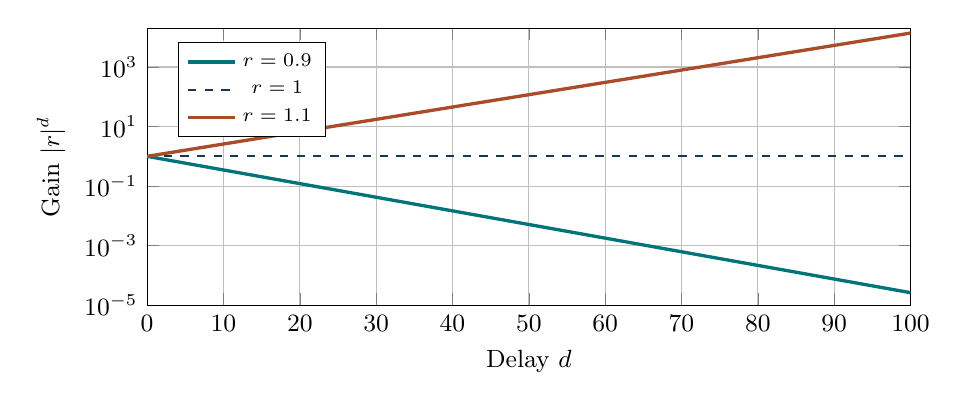
\begin{tikzpicture}
\begin{semilogyaxis}[width=0.93\linewidth,height=5.1cm,xlabel={Delay $d$},
ylabel={Gain $|r|^d$},xmin=0,xmax=100,ymin=0.00001,ymax=20000,grid=major,
ytick={0.00001,0.001,0.1,10,1000},legend style={font=\scriptsize,at={(0.04,.95)},anchor=north west},
tick label style={font=\small},label style={font=\small}]
\addplot[sea,very thick,domain=0:100]{0.9^x};\addlegendentry{$r=0.9$}
\addplot[ink,thick,dashed,domain=0:100]{1};\addlegendentry{$r=1$}
\addplot[warm,very thick,domain=0:100]{1.1^x};\addlegendentry{$r=1.1$}
\end{semilogyaxis}\end{tikzpicture}
\column{0.40\textwidth}
A scalar linear transition multiplies a perturbation by $r$ at each step:
\[
0.9^{100}\approx2.66\times10^{-5},
\]
\[
1.1^{100}\approx1.38\times10^{4}.
\]
For $0<r<1$, $r^d=e^{-d/\tau}$, with decay time $\tau=-1/\log r$ steps.
\end{columns}
\end{frame}
\begin{frame}{Saturation can shorten memory even when $W$ is large}
For a scalar $\tanh$ unit, $J_t=w(1-h_t^2)$.
For a vector state, $J_t=D_tW$, and
\[
\norm{J_t}_2\leq\norm{D_t}_2\norm{W}_2,\qquad
D_t=\diag(1-h_{t,i}^2).
\]
At $a=0$ the activation derivative is one. At $a=2$ it is about $0.0707$.
Even $w=2$ gives a local gain of only $0.141$ at that operating point.
\par
Large recurrent weights may move units into saturation. The inputs and biases
therefore matter as much as the chosen scale of $W$.
A sigmoid hidden unit has derivative at most $1/4$.
\end{frame}
\begin{frame}{Exploding gradients are directional}
For a linear recurrence, $J_t=W$ and $P_{t:k}=W^{t-k}$.
A perturbation along an eigenvector with eigenvalue $\lambda$ scales as
$\lambda^{t-k}$. Large gains can make an optimizer step excessively large.
\[
\text{For a general trajectory:}\qquad
P_{t:k}=D_tW\,D_{t-1}W\cdots D_{k+1}W.
\]
The largest singular value gives the greatest possible amplification over
this interval. The actual backward signal depends on its direction and may
remain small.
\take{An upper bound greater than one permits growth; it does not establish that a particular gradient explodes.}
\end{frame}
\begin{frame}{Stable eigenvalues can coexist with transient growth}
Consider a constant, non-normal recurrent matrix:
\[
W=\begin{pmatrix}0.9&5\\0&0.9\end{pmatrix},\qquad
W^n=\begin{pmatrix}0.9^n&5n(0.9)^{n-1}\\0&0.9^n\end{pmatrix}.
\]
Both eigenvalues equal $0.9$. Nevertheless, the upper-right entry at $n=10$
is $50(0.9)^9\approx19.37$, so an input in the second coordinate produces a
large transient in the first.
\par
Eventually $W^n$ decays. The transient demonstrates why the spectral radius
alone is a poor finite-horizon diagnostic. In a nonlinear network, the
successive Jacobians also depend on the input trajectory.
\end{frame}

\begin{frame}{Remembering an input competes with rejecting noise}
Suppose $f$ is contractive in its state for the same input:
\[
\norm{f(h,x)-f(\tilde h,x)}\leq\rho\norm{h-\tilde h},\qquad 0\leq\rho<1.
\]
If two histories differ at $k$ but receive identical inputs afterwards,
\[
\norm{h_t-\tilde h_t}\leq \rho^{t-k}\norm{h_k-\tilde h_k}.
\]
Contraction suppresses errors in the initial state. It also suppresses the
difference between two early cues that should lead to different predictions.
\par
A finite-dimensional, finite-precision state must preserve useful distinctions
while new observations arrive. Increasing $H$ creates more possible directions,
but does not guarantee that training learns a persistent one.
\end{frame}
\begin{frame}{Gradient clipping and initialization solve different problems}
For the concatenated gradient $g$ and threshold $c_*>0$, use
\[
\tilde g=\begin{cases}
g,&\norm g_2\leq c_*,\\
(c_*/\norm g_2)g,&\norm g_2>c_*.
\end{cases}
\]
Clipping preserves direction and bounds a plain SGD step by $\eta c_*$.
It does not restore a vanished contribution from a distant event.
\par
Orthogonal initialization preserves norms in a \emph{linear} recurrence.
For a $\tanh$ cell, $D_t$ can still contract the signal; unconstrained updates
can also destroy orthogonality. Check input scale and saturation alongside $W$.
\src{Week 6 handwritten notes, p.\ 13. See also Pascanu, Mikolov and Bengio (2013).}
\end{frame}
\begin{frame}{Full BPTT: arithmetic, storage and sequential work}
For a dense cell with input width $d$, hidden width $H$ and output width $p$,
\[
\text{forward and backward work per sequence}
=O\!\left(T(Hd+H^2+pH)\right).
\]
Storing the hidden states for a direct reverse sweep uses $O(TH)$ space,
in addition to parameters, inputs, outputs and other cached activations.
\par
Within a time step, matrix operations parallelize. Across time, $h_t$ must be
available before $h_{t+1}$ can be computed. Batching independent sequences
does not remove this dependence.
\par
Checkpointing saves selected states and recomputes intervening ones during
the backward pass. It can preserve the full derivative while trading compute
for memory.
\end{frame}
\begin{frame}{Truncated BPTT: what a boundary removes}
Suppose $T=6$ and chunks have length three. At the boundary carry forward
$\tilde h_3=\operatorname{stopgrad}(h_3)$: its value equals $h_3$, but its
derivative with respect to how that value was computed is zero.
\[
\underbrace{h_1,h_2,h_3}_{\text{chunk 1}}\quad
\underbrace{h_4,h_5,h_6}_{\text{chunk 2}} .
\]
A final loss at $t=6$ still uses information in $\tilde h_3$; it supplies no
gradient across that boundary to the parameter uses at $t=1,2,3$.
The uses of the shared parameters at $t=4,5,6$ still receive gradients.
\par
Truncation reduces storage per update but generally changes the gradient.
How much it changes depends on the omitted temporal paths.
\end{frame}
\begin{frame}{Carrying a state, detaching it, or resetting it}
\begin{center}\begin{tabular}{lll}\toprule
At a boundary & Numerical state & Gradient path to earlier steps\\\midrule
Carry with history & Preserved & Preserved\\
Carry and detach & Preserved & Cut\\
Reset to $h_0$ & Reinitialized & Cut\\\bottomrule
\end{tabular}\end{center}
Carry a state only between consecutive chunks of the same trajectory.
Reset between independent examples, or a batch can accidentally pass one
sequence's history into another.
\par
For variable lengths, a zero loss weight removes direct supervision at a padded
step. It does not freeze the state. Stop at the true length or explicitly
preserve the last valid state when padding.
\end{frame}
\begin{frame}{Why a good one-step fit can fail in a rollout}
At training time the model may receive measured states, whereas a free
rollout feeds back its own predictions. For a fixed forcing sequence,
define $e_t=\hat s_t-s_t$ and the local model discrepancy
$r_t=\hat f(s_t,F_t)-f(s_t,F_t)$. To first order,
\[
e_{t+1}\simeq J_{\hat f}(s_t,F_t)e_t+r_t .
\]
The rollout both injects new error and transports old error. A small one-step
test loss alone does not establish accurate phase, amplitude or timing over
many oscillator periods.
\par
Validate on held-out trajectories. Plot error against forecast horizon and
compare one-step evaluation with free rollout under the same forcing.
\end{frame}
\begin{frame}{The integrator itself can amplify errors}
For the undamped, unforced oscillator, the continuous state matrix has
eigenvalues $\pm i\omega$ with $\omega=\sqrt{k/m}$. Forward Euler has
discrete eigenvalues
\[
1\pm i\omega\Delta t,\qquad |1\pm i\omega\Delta t|
=\sqrt{1+(\omega\Delta t)^2}>1.
\]
Its amplitude grows even though the exact motion is bounded. A model that
learns the Euler update perfectly can reproduce this artificial growth.
\par
Comparing an RNN rollout against a trusted reference trajectory helps
distinguish an error in the learned dynamics from an error already present
in the training integrator.
\end{frame}
\begin{frame}{A diagnostic for each failure mode}
\small
\begin{center}\begin{tabular}{p{4.4cm}p{8.1cm}}\toprule
Observation & Measurement or controlled comparison\\\midrule
Only short-delay cases work & Vary the delay on the copy task. Track the final loss gradient at each earlier state.\\[3pt]
Loss spikes intermittently & Log the global gradient norm before clipping, the clipping fraction and update norms.\\[3pt]
Many hidden units are near $\pm1$ & Inspect the distribution of $1-h_{t,i}^2$ and rescale the inputs if appropriate.\\[3pt]
Results depend on chunk boundaries & Vary chunk length while keeping the task and loss normalization fixed.\\[3pt]
One-step errors are small but rollouts drift & Compare phase and amplitude over increasing horizons on held-out trajectories.\\\bottomrule
\end{tabular}\end{center}
\end{frame}
\section{Implementation and exercises}
\begin{frame}[fragile]{NumPy: forward pass with a weighted regression loss}
\begin{lstlisting}
import numpy as np

def loss_and_grads(X, Y, p, h0, alpha):
    U, W, V, b, c = [p[k] for k in ("U","W","V","b","c")]
    h = [np.array(h0, dtype=float, copy=True)]
    o = []
    for xt in X:
        h.append(np.tanh(U @ xt + W @ h[-1] + b))
        o.append(V @ h[-1] + c)
    r = np.asarray(o) - Y
    loss = 0.5 * np.sum(alpha[:, None] * r**2)
\end{lstlisting}
$X$ has shape $(T,d)$ and $Y$ has shape $(T,p)$. The weights \texttt{alpha}
have shape $(T,)$. The initial state occupies \texttt{h[0]}.
\end{frame}
\begin{frame}[fragile]{NumPy: reverse pass and gradient accumulation}
\begin{lstlisting}
    grads = {k: np.zeros_like(a) for k, a in p.items()}
    carry = np.zeros_like(h[0])
    for t in reversed(range(len(X))):
        e = alpha[t] * r[t]
        grads["V"] += np.outer(e, h[t+1])
        grads["c"] += e
        da = (V.T @ e + carry) * (1.0 - h[t+1]**2)
        grads["W"] += np.outer(da, h[t])
        grads["U"] += np.outer(da, X[t])
        grads["b"] += da
        carry = W.T @ da
    return loss, grads, carry
\end{lstlisting}
In Python, \texttt{h[t]} is the state \emph{before} reading \texttt{X[t]}.
After the loop, \texttt{carry} equals $\nabla_{h_0}\mathcal L$.
\end{frame}
\begin{frame}{Exercises for the lecture}
\begin{enumerate}
\item For a $64\times64\times3$ input with $K=16$, $F=5$, $S=2$, $P=2$,
calculate the output shape and the number of trainable parameters.
\item Take $\phi(a)=a$. Write out $h_3$ in terms of $x_1,x_2,x_3,h_0$ for
$b=0$. Which power of $W$ multiplies $Ux_1$?
\item In the two-step scalar example, set $w=0$. Which of the gradients
$\partial\mathcal L/\partial u$ and $\partial\mathcal L/\partial w$ vanishes?
\item Fit the oscillator with forcing on held-out trajectories. Compare
full and truncated BPTT as the delay between observations increases.
\end{enumerate}
\end{frame}
\begin{frame}{Checks on the first three exercises}
\begin{enumerate}
\item $1+\lfloor(64+4-5)/2\rfloor=32$. The output shape is $32\times32\times16$.
There are $16(5^2\cdot3+1)=1216$ parameters.
\item $h_3=W^3h_0+W^2Ux_1+WUx_2+Ux_3$. Earlier inputs pass through more
applications of $W$.
\item With $w=0$, $h_2=0$, $e_2=-0.5$ and $\delta_2=-0.5$. Hence
\[
\partial_u\mathcal L=0,\qquad
\partial_w\mathcal L=\delta_2h_1=-0.5\tanh(1)\approx-0.380797 .
\]
The loss cannot teach the input weight $u$ through a zero recurrent link in
this example, yet it can teach the link itself to change.
\end{enumerate}
\end{frame}
\begin{frame}{Source notes and further reading}
\textbf{Handwritten lecture notes: FYS5429/9429.}
\emph{Notesweek4.pdf} (February 12), pp.\ 1--10: convolutional stages,
filter examples, padding and stride. \emph{Notesweek5.pdf} (February 19),
pp.\ 1--6: oscillator dynamics and the learning objective. \\ \emph{Notesweek6.pdf} (February 27), pp.\ 1--13: the RNN cell, BPTT, eigenmodes and clipping.
\par\medskip
\textbf{Recurrent computation and BPTT.}
I. Goodfellow, Y. Bengio and A. Courville, \emph{Deep Learning}, MIT Press
(2016), \href{https://www.deeplearningbook.org/contents/rnn.html}{Chapter 10}.
\par\medskip
\textbf{Temporal gradients and clipping.}
R. Pascanu, T. Mikolov and Y. Bengio,
\href{https://proceedings.mlr.press/v28/pascanu13.html}{On the difficulty of training recurrent neural networks},
ICML, PMLR 28(3), 1310--1318 (2013).
\end{frame}
\end{document}

